%================================================================
\section{Method}\label{sec:Method}
%================================================================

%----------------------------------------------------------------
\subsection{The Heat Equation Problem}\label{sec:heat method}
%----------------------------------------------------------------

Following the discussion in \autoref{sec:Heat numerical Theory}, the computational algorithm \cite{hpl} for the Forward Euler explicit scheme becomes:
\begin{enumerate}
    \item Compute $u_i^0 = I(x)$ for $i=0, ..., N_x$
    \item for $n=0,1, ..., N_t$:
        \begin{itemize}
            \item[(a)] apply \autoref{eq:FE scheme} for all the internal spatial points $i=1, ..., N_x - 1$
            \item[(b)] set the boundary values $u_i^{n+1}=0$ for $i=0$ and $i=N_x$.
        \end{itemize}
\end{enumerate}


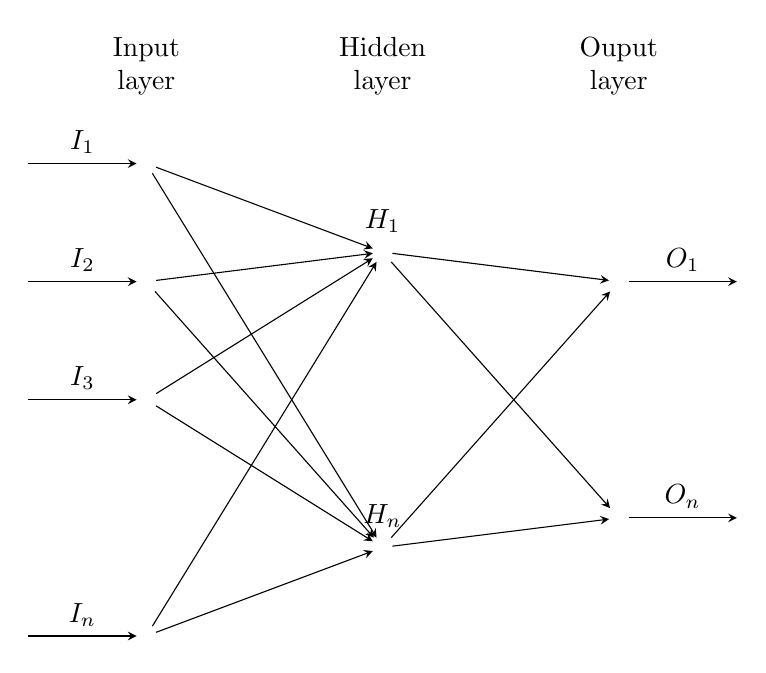
\begin{tikzpicture}[x=1.5cm, y=1.5cm, >=stealth]

\foreach \m/\l [count=\y] in {1,2,3,missing,4}
  \node [every neuron/.try, neuron \m/.try] (input-\m) at (0,2.5-\y) {};

\foreach \m [count=\y] in {1,missing,2}
  \node [every neuron/.try, neuron \m/.try ] (hidden-\m) at (2,2-\y*1.25) {};

\foreach \m [count=\y] in {1,missing,2}
  \node [every neuron/.try, neuron \m/.try ] (output-\m) at (4,1.5-\y) {};

\foreach \l [count=\i] in {1,2,3,n}
  \draw [<-] (input-\i) -- ++(-1,0)
    node [above, midway] {$I_\l$};

\foreach \l [count=\i] in {1,n}
  \node [above] at (hidden-\i.north) {$H_\l$};

\foreach \l [count=\i] in {1,n}
  \draw [->] (output-\i) -- ++(1,0)
    node [above, midway] {$O_\l$};

\foreach \i in {1,...,4}
  \foreach \j in {1,...,2}
    \draw [->] (input-\i) -- (hidden-\j);

\foreach \i in {1,...,2}
  \foreach \j in {1,...,2}
    \draw [->] (hidden-\i) -- (output-\j);

\foreach \l [count=\x from 0] in {Input, Hidden, Ouput}
  \node [align=center, above] at (\x*2,2) {\l \\ layer};

\end{tikzpicture}

%====================
%====================

\def\layersep{3cm}
\def\nodeinlayersep{1.5cm}
\begin{tikzpicture}[
   shorten >=1pt,->,
   draw=black!50,
    node distance=\layersep,
    every pin edge/.style={<-,shorten <=1pt},
    neuron/.style={circle,fill=black!25,minimum size=17pt,inner sep=0pt},
    input neuron/.style={neuron, fill=green!50},
    output neuron/.style={neuron, fill=red!50},
    hidden neuron/.style={neuron, fill=blue!50},
    annot/.style={text width=4em, text centered}
]
    % Draw the input layer nodes
    \foreach \name / \y in {1,...,3}
    % This is the same as writing \foreach \name / \y in {1/1,2/2,3/3,4/4}
        \node[input neuron, pin=left:Input \#\y] (I-\name) at (0,-\y) {};
    % set number of hidden layers
    \newcommand\Nhidden{2}
    % Draw the hidden layer nodes
    \foreach \N in {1,...,\Nhidden} {
       \foreach \y in {1,...,12} {
          \path[yshift=6cm]
          node[hidden neuron] (H\N-\y) at (\N*\layersep,-\y*\nodeinlayersep ) {$\frac{1}{1+e^{-x}}$};
           }
    \node[annot,above of=H\N-1, node distance=1cm] (hl\N) {Hidden layer \N};
    }
    % Draw the output layer node
    \node[output neuron,pin={[pin edge={->}]right:Output}, right of=H\Nhidden-6] (O) {};
%
    % Connect every node in the input layer with every node in the
    % hidden layer.
    \foreach \source in {1,...,3}
        \foreach \dest in {1,...,12}
            \path (I-\source) edge (H1-\dest);
    % connect all hidden stuff
    \foreach [remember=\N as \lastN (initially 1)] \N in {2,...,\Nhidden}
       \foreach \source in {1,...,12}
           \foreach \dest in {1,...,12}
               \path (H\lastN-\source) edge (H\N-\dest);
    % Connect every node in the hidden layer with the output layer
    \foreach \source in {1,...,12}
        \path (H\Nhidden-\source) edge (O);
    % Annotate the layers
    \node[annot,left of=hl1] {Input layer};
    \node[annot,right of=hl\Nhidden] {Output layer};
\end{tikzpicture}

%=====================
%=====================

%----------------------------------------------------------------
\subsection{The Eigenvalue Problem}\label{sec:eigen method}
%----------------------------------------------------------------


In this notebook, a FFNN model is employed to learn the solution to the nonlinear, coupled ODE, presented by Yi et. al in \cite{yfh04}, describing the state of a CTRNN model. Given a real symmetric matrix $A$ in the source term, the temporal dynamic described by this ODE has convergence properties to the largest eigenvalue. Simply replacing $A$ with $-A$ yield the smallest eigenvalue

The article also states that the network should converge to a different eigenvalue if the initial vector, $\mathbf{x}_0$, is orthogonal to the eigenvector corresponding to the largest eigenvalue.

FFNN model is employed within the \cw{TensorFlow} framework


The aim is to design a FFNN model suitable for solving this ODE, and check if it succeed in computing both the largest and smallest eigenvalue for some benchmark $3\times 3$ and $6\times 6$ real symmetric matrices. We will also check whether the network converges to a different eigenvalue than the largest if $\mathbf{x}_0$ is chosen to be orthogonal to the eigenvector corresponding to the largest eigenvalue. 

In order to assess the FFNN model, we will compare the result with those from Euler's method for solving the same ODE and  \cw{Numpy's linalg.eig} which directly computes the eigenvalues of the matrix $A$.